\documentclass[convert={density=300,size=1080x800,outext=.png}]{standalone}
\usepackage{xcolor}
\usepackage{graphics, graphicx}
\usepackage{tikz, tkz-graph}
\usepackage{pgf, pgfplots}
\usepackage{graphviz, tkz-berge}
\usepackage{graphics, graphicx}
\usepackage{pstricks, pst-node, pst-tree}

\usetikzlibrary{arrows, petri, topaths}
\usetikzlibrary{shapes}
\usetikzlibrary{arrows.meta}
\usetikzlibrary{positioning,automata}



\begin{document}
		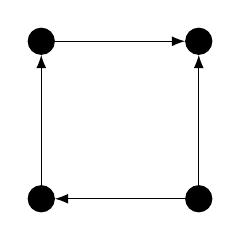
\begin{tikzpicture}[round/.style={circle, draw=black, fill=black, thin, minimum size=1mm}, transform shape]
			\node[round] (a) at (0,0){};
			\node[round] (b) at (0,2) {};
			\node[round] (c) at (2,0) {};
			\node[round] (d) at (2,2) {};
			\draw (a) edge[->, -Latex] (b);
			\draw (c) edge[->, -Latex] (a);
			\draw (b) edge[->, -Latex] (d);
			\draw (c) edge[->, -Latex] (d);
		\end{tikzpicture}
\end{document}